\subsection{The Cleaning Service}
\label{sec:cleaningService}

Deliverable 3.2~\cite{d3.2} presents a description of the RESTful API of the cleaning service. 
The cleaning service contains the two methods \texttt{getCleaningSuggestions} and \texttt{clean}, of which we give an update.
The functionality of the methods  declared in the Deliverable 3.1~\cite{d3.1} remains unchanged. 
\todo{@Ruslan please write about changes from  POST to REST and why}

The typical usage of the cleaning service follows the workflow outlined for the cleaning application in figure \ref{fig:workflow}.
The updated user interface is shown in figure \ref{fig:ui}

\begin{figure}[ht!]
\centering
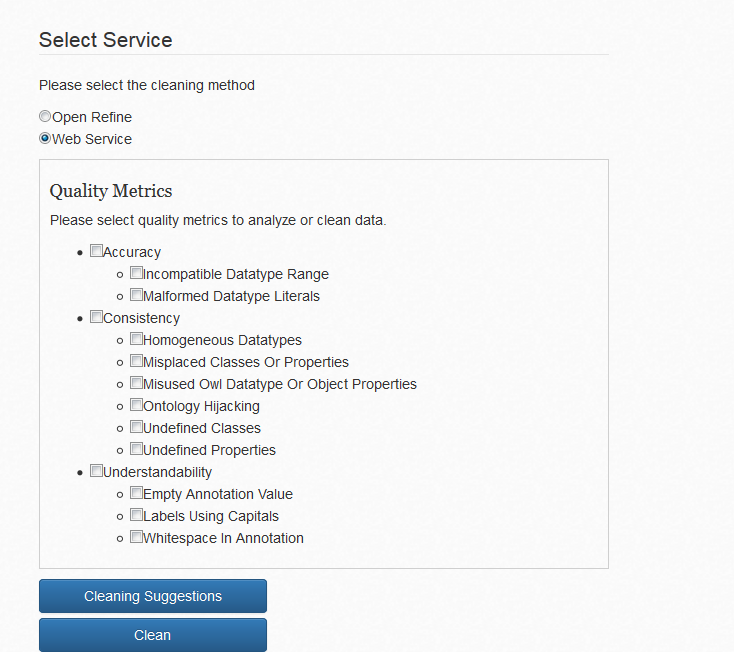
\includegraphics[width=\textwidth]{figures/WebService.png}
\caption{Cleaning process workflow}
\label{fig:ui}
\end{figure}





\subsubsection{Exposed Web Service Interfaces}
\label{sec:service-API}


\begin{table}[h]
\captionsetup{justification=raggedright,singlelinecheck=false}
\caption{Cleaning Methods}
\label{tbl:valid_meth}
\begin{tabular}{|p{5cm}|p{10cm}|}
\hline
\multicolumn{2}{|l|}{\textbf{Methods}} \\ \hline

\textbf{Modifier and Type} & 
\textbf{Method and Description} \\ \hline

\texttt{javax.ws.rs.core.Response} & 
\texttt{getCleaningSuggestionsJSON(java.lang.String inputMessage)}:
\textbf{REST} method which returns a set of cleaning suggestions. \\ \hline

\texttt{javax.ws.rs.core.Response} & 
\texttt{cleanJSON(java.lang.String inputMessage)}:
\textbf{REST} method which removes triples affected by selected quality problems). \\ \hline

\hline
\end{tabular}
\end{table}

\subparagraph{Method Details}

\begin{description}

\item{\textbf{getCleaningSuggestionsJSON}:} \textbf{REST} method which returns a set of cleaning suggestions.

\textbf{URL (partial):} \url{/quality_extension/get_cleaning_suggestions} 

\textbf{Parameters}: 
\begin{itemize}
\item \texttt{inputMessage}: A JSON-encoded string which has the following form: \\
\{ \\
\hspace*{0.5 cm}"download":"Dataset", \\
\hspace*{0.5 cm}"metrics":["metric1", "metric2"], \\ 
\} \\
\end{itemize}
where : 
\begin{description}
\item[Dataset:] The URI of a file to be validated. 
\item[MetricsConfiguration:] a list of quality metrics metrics is list of metrics with respect to which cleaning suggestions should be generated. 
\end{description}




\textbf{Returns}: A Response instance which has a JSON-encoded entity content depending on the input parameter of the method. We discriminate the following cases: 
\begin{itemize}
\item  \{"status":"error","message":"Request parameters are not complete.\} when the input parameter are not correct. 
\item  Cleaning report -  a set of triples containing cleaning suggestions serialized as TURTLE string in the case of success.
\end{itemize}
The cleaning report is created according to the QR (Quality Report) and QPROB (Quality Problems) ontologies presented in Deliverable 3.2~\cite{d3.2}.
An example of the cleaning report is shown in Figure \ref{lst:cleaning_report}.


We also extended cleaning report by statistics that summarize information about identified quality problems and affected triples. 
The QR ontologie were extended by the corresponding classes and properties represented in Figure \ref{fig:stat}

\lstinputlisting[caption={An example of a cleaning report},label=lst:cleaning_report]{figures/cleaning_report.trig}

\begin{figure}[ht!]
\centering
\includegraphics[page=8,trim=1.0cm 1.0cm 1.0cm 1.0cm,clip,width=\textwidth]{figures/CleaningFigures.pdf}
\caption{Quality Statistics in Quality Report Ontology}
\label{fig:qstat}
\end{figure}

\item{\textbf{cleanJSON}:} \textbf{POST} method which which cleans a dataset by applying the rule ``delete every triple that is affected by a quality problem w.r.t.\ to at least one of the metrics specified''.

\textbf{URL (partial):} \url{/diachron/clean} 

\textbf{Parameters}: 
\begin{itemize}
\item \texttt{inputMessage}: A JSON-encoded string which has the following form: \\
\{ \\
\hspace*{0.5 cm}"download":"Dataset", \\
\hspace*{0.5 cm}"metrics":["metric1", "metric2"], \\ 
\} \\


\begin{description}
\item[Dataset:] The URI of an RDF file to be validated. 
\item[metrics:]  is list of metrics with respect to which cleaning suggestions should be 		generated.
\end{description}
\end{itemize}
\textbf{Returns}: A Response instance which has a JSON-encoded entity content depending on the input parameter of the method. We discriminate the following cases: 
\begin{itemize}
\item  \{"status":"error","message":"Request parameters are not complete.\}
\item The following JSON string:
\{ \\
\hspace*{0.5 cm}"uri":"cleaned document", \\
\hspace*{0.5 cm}"delta":"delta document" \\ 
\} \\
if the input parameter has the correct form where:
\begin{description}
\item [uri:] is cleaned document serialized as TURTLE string.
\item [Delta:] delta represents changes done in original document inorder to clean it, serialized as 	TURTLE.
\end{description} 
\end{itemize}

\end{description}






\

%%% Local Variables: 
%%% mode: latex
%%% TeX-master: "D3.2"
%%% End: 
